\documentclass{beamer}

% This file is a solution template for:

% - Giving a talk on some subject.
% - The talk is between 15min and 45min long.
% - Style is ornate.



% Copyright 2004 by Till Tantau <tantau@users.sourceforge.net>.
%
% In principle, this file can be redistributed and/or modified under
% the terms of the GNU Public License, version 2.
%
% However, this file is supposed to be a template to be modified
% for your own needs. For this reason, if you use this file as a
% template and not specifically distribute it as part of a another
% package/program, I grant the extra permission to freely copy and
% modify this file as you see fit and even to delete this copyright
% notice. 


\mode<presentation>
{
  \usetheme{Warsaw}
  % or ...

  \setbeamercovered{transparent}
  % or whatever (possibly just delete it)
}


\usepackage[english]{babel}
% or whatever

\usepackage[utf8]{inputenc}
% or whatever

\usepackage{times}
\usepackage[T1]{fontenc}
% Or whatever. Note that the encoding and the font should match. If T1
% does not look nice, try deleting the line with the fontenc.

\usepackage{pgfgantt}

\title[Restraint Selection in PSP] % (optional, use only with long paper titles)
{Improve the use of noisy restraints in ab initio protein structure prediction}

%\subtitle
%{Presentation Subtitle} % (optional)

\author%[Author, Another] % (optional, use only with lots of authors)
{David Lassner, Marius Knaust, Moritz Neeb}
% - Use the \inst{?} command only if the authors have different
%   affiliation.

\institute[Universities of Somewhere and Elsewhere] % (optional, but mostly needed)
{
  Computational Biology Project\\
  TU Berlin}
% - Use the \inst command only if there are several affiliations.
% - Keep it simple, no one is interested in your street address.

\date%[Short Occasion] % (optional)
{Nov 28, 2014}

\subject{Talks}
% This is only inserted into the PDF information catalog. Can be left
% out. 



% If you have a file called "university-logo-filename.xxx", where xxx
% is a graphic format that can be processed by latex or pdflatex,
% resp., then you can add a logo as follows:

% \pgfdeclareimage[height=0.5cm]{university-logo}{university-logo-filename}
% \logo{\pgfuseimage{university-logo}}



% Delete this, if you do not want the table of contents to pop up at
% the beginning of each subsection:
%\AtBeginSubsection[]
%{
%  \begin{frame}<beamer>{Outline}
%    \tableofcontents[currentsection,currentsubsection]
%  \end{frame}
%}


% If you wish to uncover everything in a step-wise fashion, uncomment
% the following command: 

%\beamerdefaultoverlayspecification{<+->}


\begin{document}

\begin{frame}
  \titlepage
\end{frame}

\begin{frame}{Outline}
  \tableofcontents
  % You might wish to add the option [pausesections]
\end{frame}


% Since this a solution template for a generic talk, very little can
% be said about how it should be structured. However, the talk length
% of between 15min and 45min and the theme suggest that you stick to
% the following rules:  

% - Exactly two or three sections (other than the summary).
% - At *most* three subsections per section.
% - Talk about 30s to 2min per frame. So there should be between about
%   15 and 30 frames, all told.

\section{Problem Description}

\begin{frame}{Structure Prediction with contact restraints}{Background}

\begin{itemize}
    \item Goal: secondary $\rightarrow$ tertiary
    \item Use of contact points reduces complexity of search space
\end{itemize}
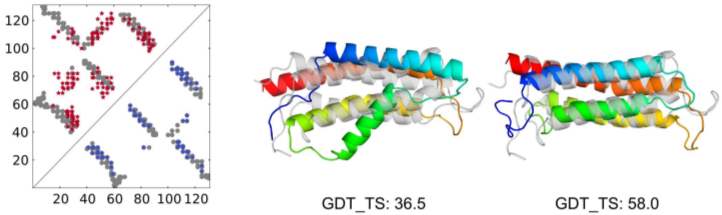
\includegraphics[width=\textwidth]{contact_prediction}\footnote{from Schneider, Brock -- 
Combining Physicochemical and Evolutionary
Information for Protein Contact Prediction}
\end{frame}

\begin{frame}{Structure Prediction with contact restraints}{Pipeline}
\begin{enumerate}
    \item Get restraints as input
    % explain contact restraints: 8Å
    \item Update energy function
    % show on whiteboard
    \item Run Monte Carlo with Metropolis Criterion
\end{enumerate}
$\Rightarrow$ \emph{guided search}, cf. MBS/MIMIC
%The search is thus guided by employment of the information from the constraints. In what way is this \emph{guiding} comparable to methods in MBS or MIMIC?
\end{frame}

\section{Improve the use of noisy restraints}

\begin{frame}{Improve the use of noisy restraints}{Problem}
How to make use of predicted restraints?
\begin{itemize}
    \item source of information! $\rightarrow$ reliability?
    \item tradeoff between \emph{exploration} and \emph{exploitation}
\end{itemize}
\end{frame}

\begin{frame}{Improve the use of noisy restraints}{Approach}
\begin{itemize}
    \item compatibility of restraints
    \item heuristics to group restraints
    \begin{itemize}
        \item use secondary structure
        \item use distance on primary structure
        % Show sketches on board
    \end{itemize}
    \item exploratory parameter analysis
    % compare with ground truth
\end{itemize}
\end{frame}

\section{Planning}

\begin{frame}{Project Timeline}
\begin{itemize}
\item project runs for 8 weeks: 48 -- 3
\item kickoff: today (Week 48)
    \begin{itemize}
    \item implement restraint grouping
    \end{itemize}
\item milestone I: 12. December (Week 50)
    \begin{itemize}
    \item optimize use of restraints
    \item evaluate and compare algorithms
    \end{itemize}
\item milestone II: 9th January (Week 2)
    \begin{itemize}
    \item create poster, analyze results
    \end{itemize}
\item final poster session: 15th January (Week 3)
\end{itemize}
\end{frame}

\end{document}